\documentclass{stdlocal}
\begin{document}
\section{Further Results} % (fold)
\label{sec:further_results}
  \begin{figure}[H]
    \center
    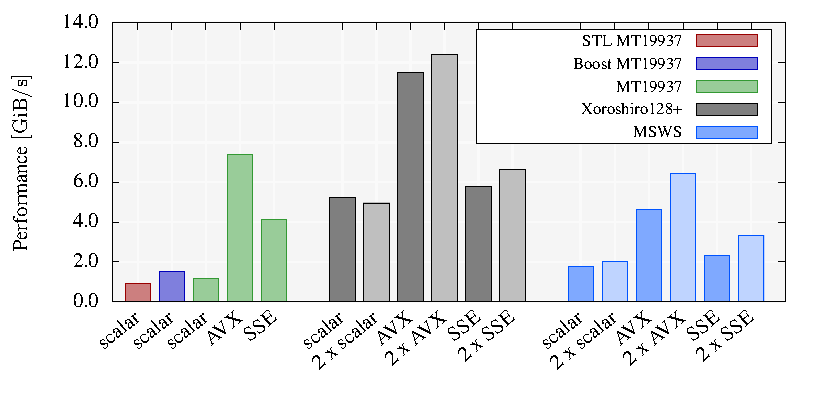
\includegraphics[width=0.95\textwidth]{plots/generation_laptop.pdf}
    \caption[Generation Benchmark Performance for \citetitle{intel-kaby-lake-i5}]{%
      The plot shows the performance resulting from the generation benchmark running on the \citetitle{intel-kaby-lake-i5} measured in $\mathrm{GiB}$ of random numbers per second for the different variants of the implemented PRNGs.
      % The prefix \enquote{2 x} states that two independent instances of the given generator were used.
      For convenience, the performances of the STL and Boost implementation of the MT19937 are shown as well.
      The data can be found in table \ref{tab:generation-data-i5}.
    }
    \label{fig:generation-performance-i5}
  \end{figure}

  \begin{figure}[H]
    \center
    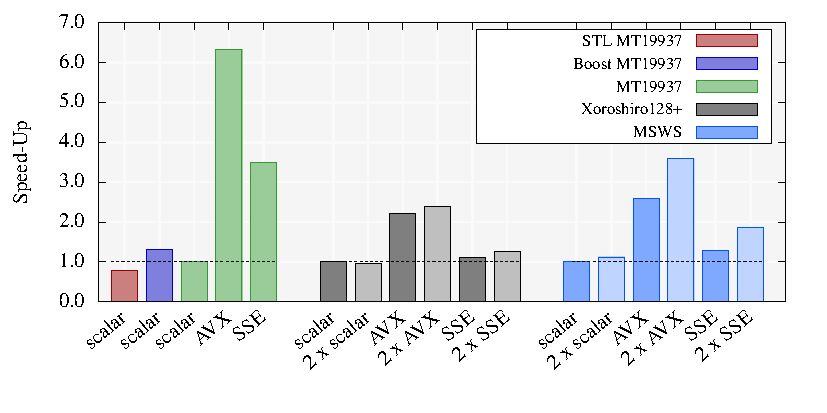
\includegraphics[width=0.95\textwidth]{plots/generation_laptop_speedup.pdf}
    \caption[Generation Benchmark Speed-Up for \citetitle{intel-kaby-lake-i5}]{%
      The plot shows the speed-up in execution time with respect to the single-instance scalar version resulting from the generation benchmark running on the \citetitle{intel-kaby-lake-i5} for the different variants of the implemented PRNGs.
      For convenience, the speed-ups of the STL and Boost implementation of the MT19937 are shown with respect to our implementation.
      The data can be found in table \ref{tab:generation-data-i5}.
    }
    \label{fig:generation-speedup-i5}
  \end{figure}

  \begin{table}[H]
    \center
    \caption[Generation Benchmark Data for \citetitle{intel-kaby-lake-i5}]{%
      The table shows the results achieved by running the generation benchmark on the \citetitle{intel-kaby-lake-i5} at a frequency of $4.51\appendUnit{GHz}$ with all implemented variants of given PRNGs.
      While running the benchmark, $16\appendUnit{GiB}$ of random numbers were generated and temporarily stored in a cache of size $16384\appendUnit{B}$ by iterating $2^{20}$ times over its content.
      During the execution, there were no cache or branch misses.
      The values for cycles, instructions, and IPCs were averaged over the calls to the advancing routine of the respective generator.
    }
    \label{tab:generation-data-i5}
    \footnotesize
    \renewcommand{\arraystretch}{1.2}
    \subimport{tables/}{generation_laptop}
  \end{table}

  \begin{figure}[H]
    \center
    \begin{subfigure}[b]{\textwidth}
      \center
      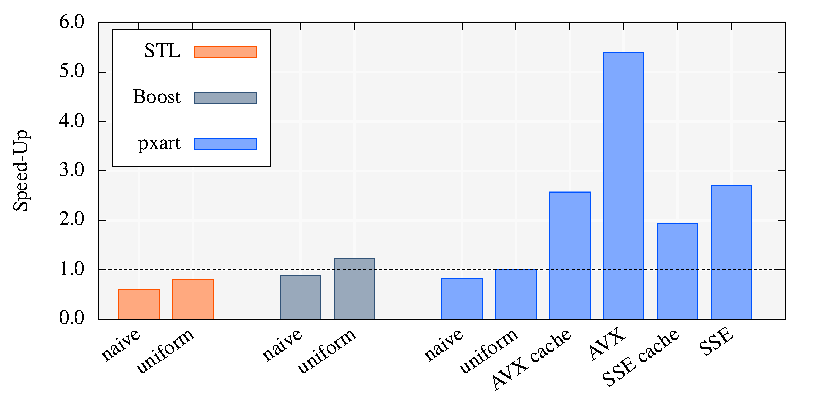
\includegraphics[width=0.95\textwidth]{plots/monte_carlo_pi_laptop_mt19937.pdf}
      \caption{MT19937}
    \end{subfigure}

    \begin{subfigure}[b]{\textwidth}
      \center
      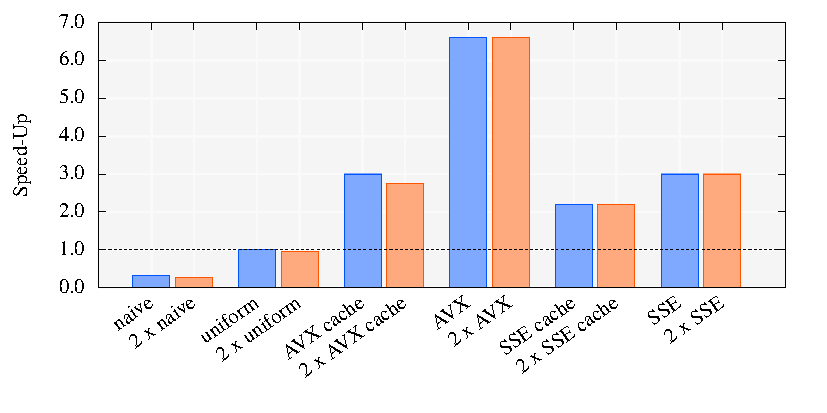
\includegraphics[width=0.95\textwidth]{plots/monte_carlo_pi_laptop_xrsr128p.pdf}
      \caption{Xoroshiro128+}
    \end{subfigure}

    \begin{subfigure}[b]{\textwidth}
      \center
      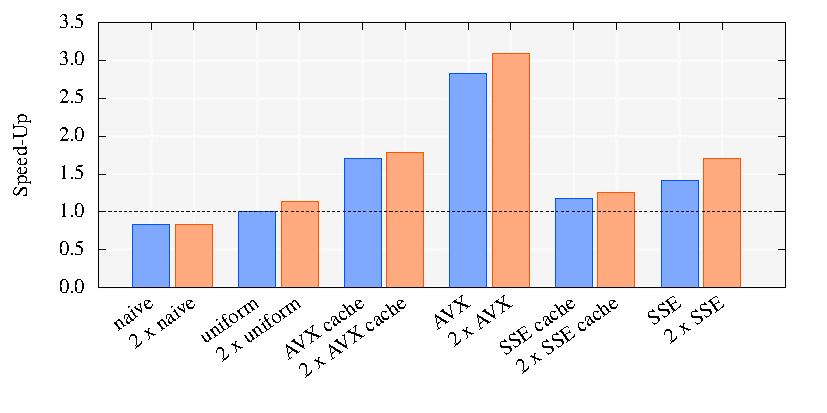
\includegraphics[width=0.95\textwidth]{plots/monte_carlo_pi_laptop_msws.pdf}
      \caption{MSWS}
    \end{subfigure}
    \caption[Monte Carlo π Benchmark Speed-Up for \citetitle{intel-kaby-lake-i5}]{%
      The plot shows the speed-up in execution time with respect to the single-instance uniform version resulting from the Monte Carlo π benchmark running on the \citetitle{intel-kaby-lake-i5} for the different variants of the implemented PRNGs and benchmark scenarios.
      For convenience, the speed-ups of the STL and Boost implementation of the MT19937 are shown with respect to our implementation.
      The data can be found in table \ref{tab:monte-carlo-pi-data-i5}.
    }
    \label{fig:monte-carlo-pi-speedup-i5}
  \end{figure}

  \begin{table}[H]
    \center
    \caption[Monte Carlo π Benchmark Data for \citetitle{intel-kaby-lake-i5}]{%
      The table shows the results achieved by running the Monte Carlo π Benchmark on the \citetitle{intel-kaby-lake-i5} with all implemented variants of given PRNGs and benchmark scenarios.
      While running the benchmark, $10^{8}$ samples in the unit square were used to estimate the value of π.
      It was ensured that the estimation error was small enough according to the calculation at the end of section \ref{sub:monte_carlo_integration}.
      During the execution, there were no cache or branch misses.
      The values for cycles, instructions, and IPCs were averaged over the number of samples in the unit square.
    }
    \label{tab:monte-carlo-pi-data-i5}
    \footnotesize
    \renewcommand{\arraystretch}{1.2}
    \subimport{tables/}{monte_carlo_pi_laptop.tex}
  \end{table}
% section further_results (end)
\end{document}